\documentclass{article}

%Les différent module pour faire des math, ou autre(un peu comme les includes en C)
\usepackage{amsmath, amssymb, amsthm}
\usepackage[french]{babel} %pour écrire en français
\usepackage[boxruled, vlined, french]{algorithm2e} %pour ecrire les programme
\usepackage{graphicx} %pour inserer des images



% Mise en page
\usepackage{geometry}
\geometry{margin=2.5cm}

%modification de certaine commande
\renewcommand{\contentsname}{Table des matières}
%modifie la configuration de base pour avoir les pseudo code en fr
\SetKwInput{KwInput}{Entrée}
\SetKwInput{KwOutput}{Sortie}
\SetKw{KwTo}{à}
\SetKw{KwRet}{retourner}
\SetKwFor{While}{Tant que}{faire}{fin tant que}
\SetKwIF{If}{ElseIf}{Else}{Si}{alors}{Sinon si}{Sinon}{fin si}
\SetKwFor{For}{Pour}{faire}{fin pour}
\SetKwFor{ForEach}{Pour chaque}{faire}{fin pour}

% Théorèmes
\newtheorem{theoreme}{Théorème}
\newtheorem{proposition}{Proposition}
\newtheorem{lemme}{Lemme}
\newtheorem{preuve}{Preuve}


\title{Titre de l'article}
\author{Votre Nom}
\date{2025-2026}

\begin{document}
    \maketitle %affiche le titre, le nom de l'autheur, ....
    \tableofcontents %creer automatiquement la table de mathière
    \newpage % fait un saut de page
    
    %le latex est un language de balisage, donc la structure est \begin{...} ici le texte \end{...}
    
    \section{Introduction} %pas d'effet visuel, structure le code et permet la génération de la table des matières
        Voici mon intro

    \section{nom I}
        \subsection{A} %créer une sous section exmple I.A)
            du texte
        \subsection{B} %I.B)
            encore du texte
        \subsection{C}
            toujours du texte
    
    \section{nom II}
        \subsection{hypothèse}
            \begin{lemme}
                blabla du lemme
            \end{lemme}
            \begin{proposition}
                blabla de la proposition
            \end{proposition}
        \subsection{theoreme}
            \begin{theoreme}
                bla bla du théorème
            \end{theoreme}
        \subsection{preuve}
            \begin{preuve}
                bla bla preuve
            \end{preuve}
        \subsection{ecrire des math}
            pour commencer une section de symbole de math faire \textbackslash[ du blabla \textbackslash]
            \\ %fait un saut de line
            \[\frac{a}{b}\]%section de math
    
    \section{Insertion image}
        \subsection{Image}
            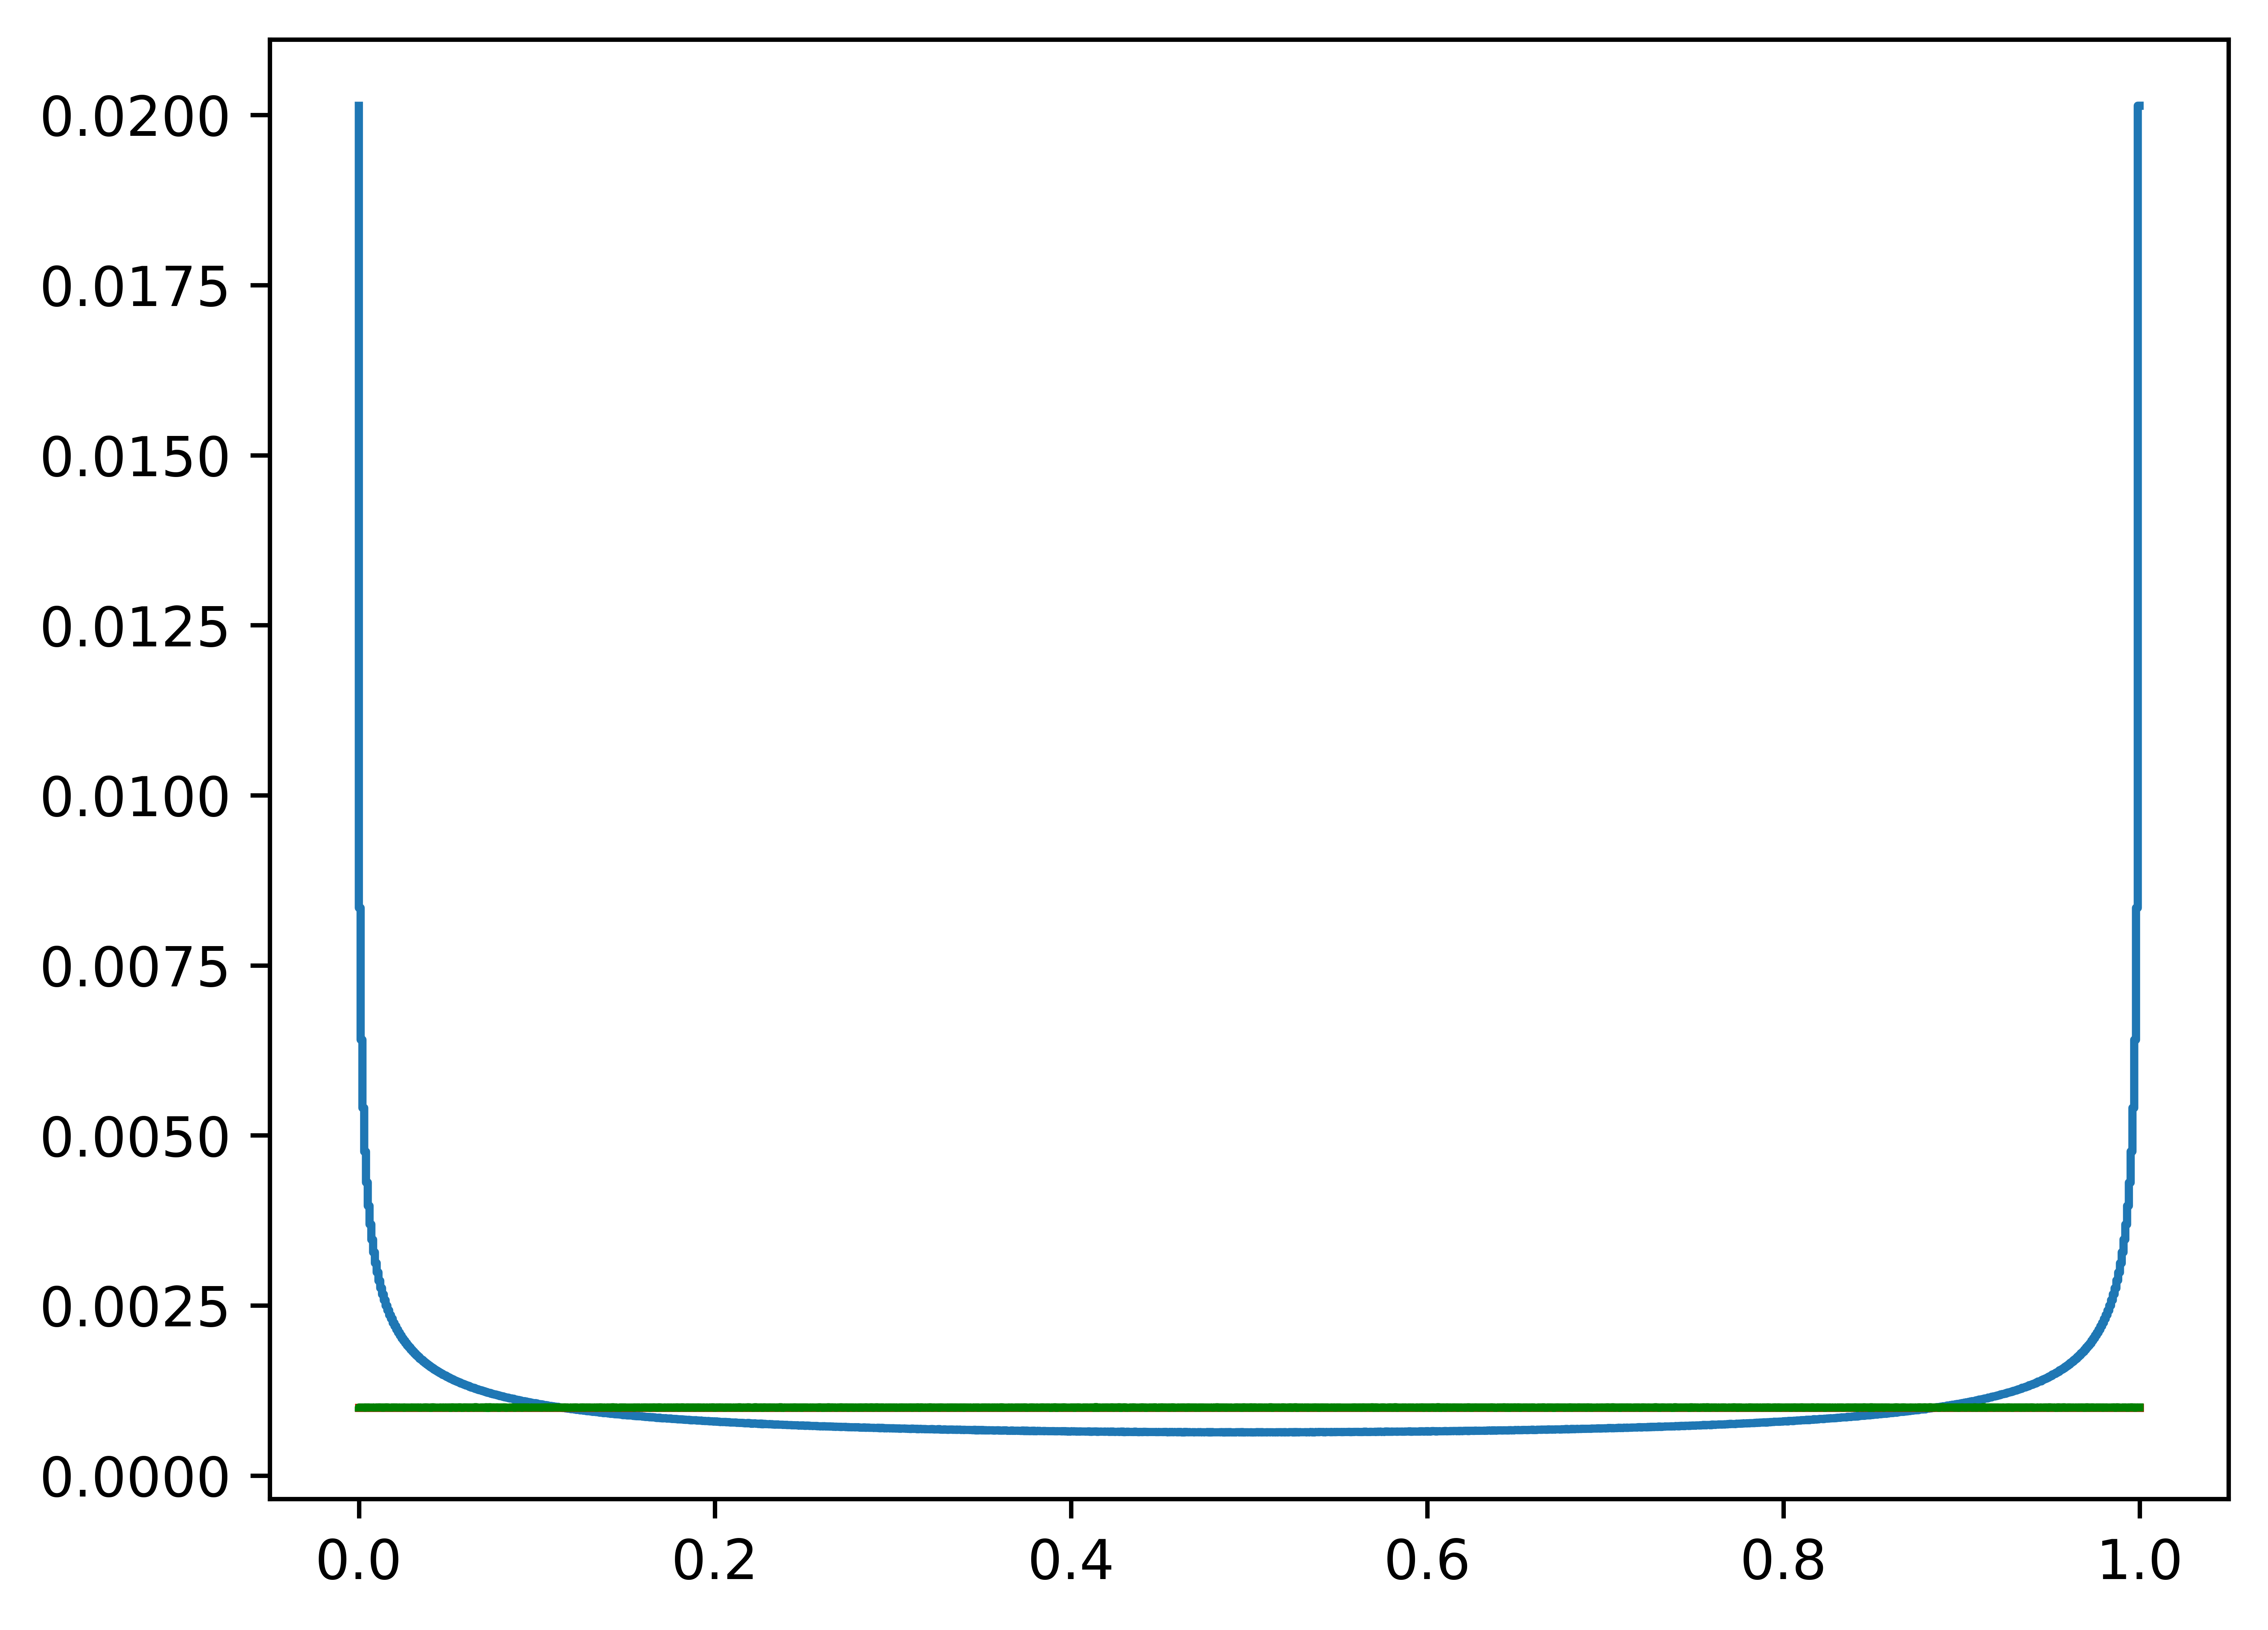
\includegraphics[scale=0.25]{image.png} %chemin vers l'image
        \subsection{Programme language naturel}
            \begin{algorithm}[H]
                \caption{Simulation de mouvement aléatoire} 

                \SetKwData{Temps}{temps}
                \SetKwData{Tf}{temps\_final}
                \SetKwData{Dt}{dt}
                \SetKwData{V}{v}
                \SetKwData{Ens}{T}
                \SetKwInOut{Input}{Entrée}

                \Input{Un ensemble de points \Ens, vitesse \V, pas de temps \Dt, \Tf}
                \BlankLine

                \Temps $\leftarrow$ 0\;
                \While{\Temps $<$ \Tf}{
                    \ForEach{point $P$ dans \Ens}{
                        Choisir $\alpha \in [0, 2\pi]$\;
                        Déplacer $P$ de la distance \V dans la direction $\alpha$\;
                    }
                    \Temps $\leftarrow$ \Temps + \Dt\;
                }
            \end{algorithm}
    
\end{document}